\section{Sistema de Monitoreo Ambiental}

El Área Metropolitana de Monterrey (AMM) se ubica en una región montañosa donde se realizan extracciones de material para la construcción (pedreras) a la par de actividades industriales y alto flujo vehicular. El Sistema de Monitoreo Ambiental (SIMA) tiene como objetivo evaluar la calidad del aire, monitoreando las concentraciones de contaminantes atmosféricos a las que se encuentra expuesta la población del AMM y, bajo condiciones adversas, advertir sobre los periodos de altos índices de contaminación atmosféria. El SIMA se compone de 13 estaciones de monitoreo repartidas a lo largo del AMM (figura \ref{fig:stations}).

\begin{figure}[H]
	\centering
	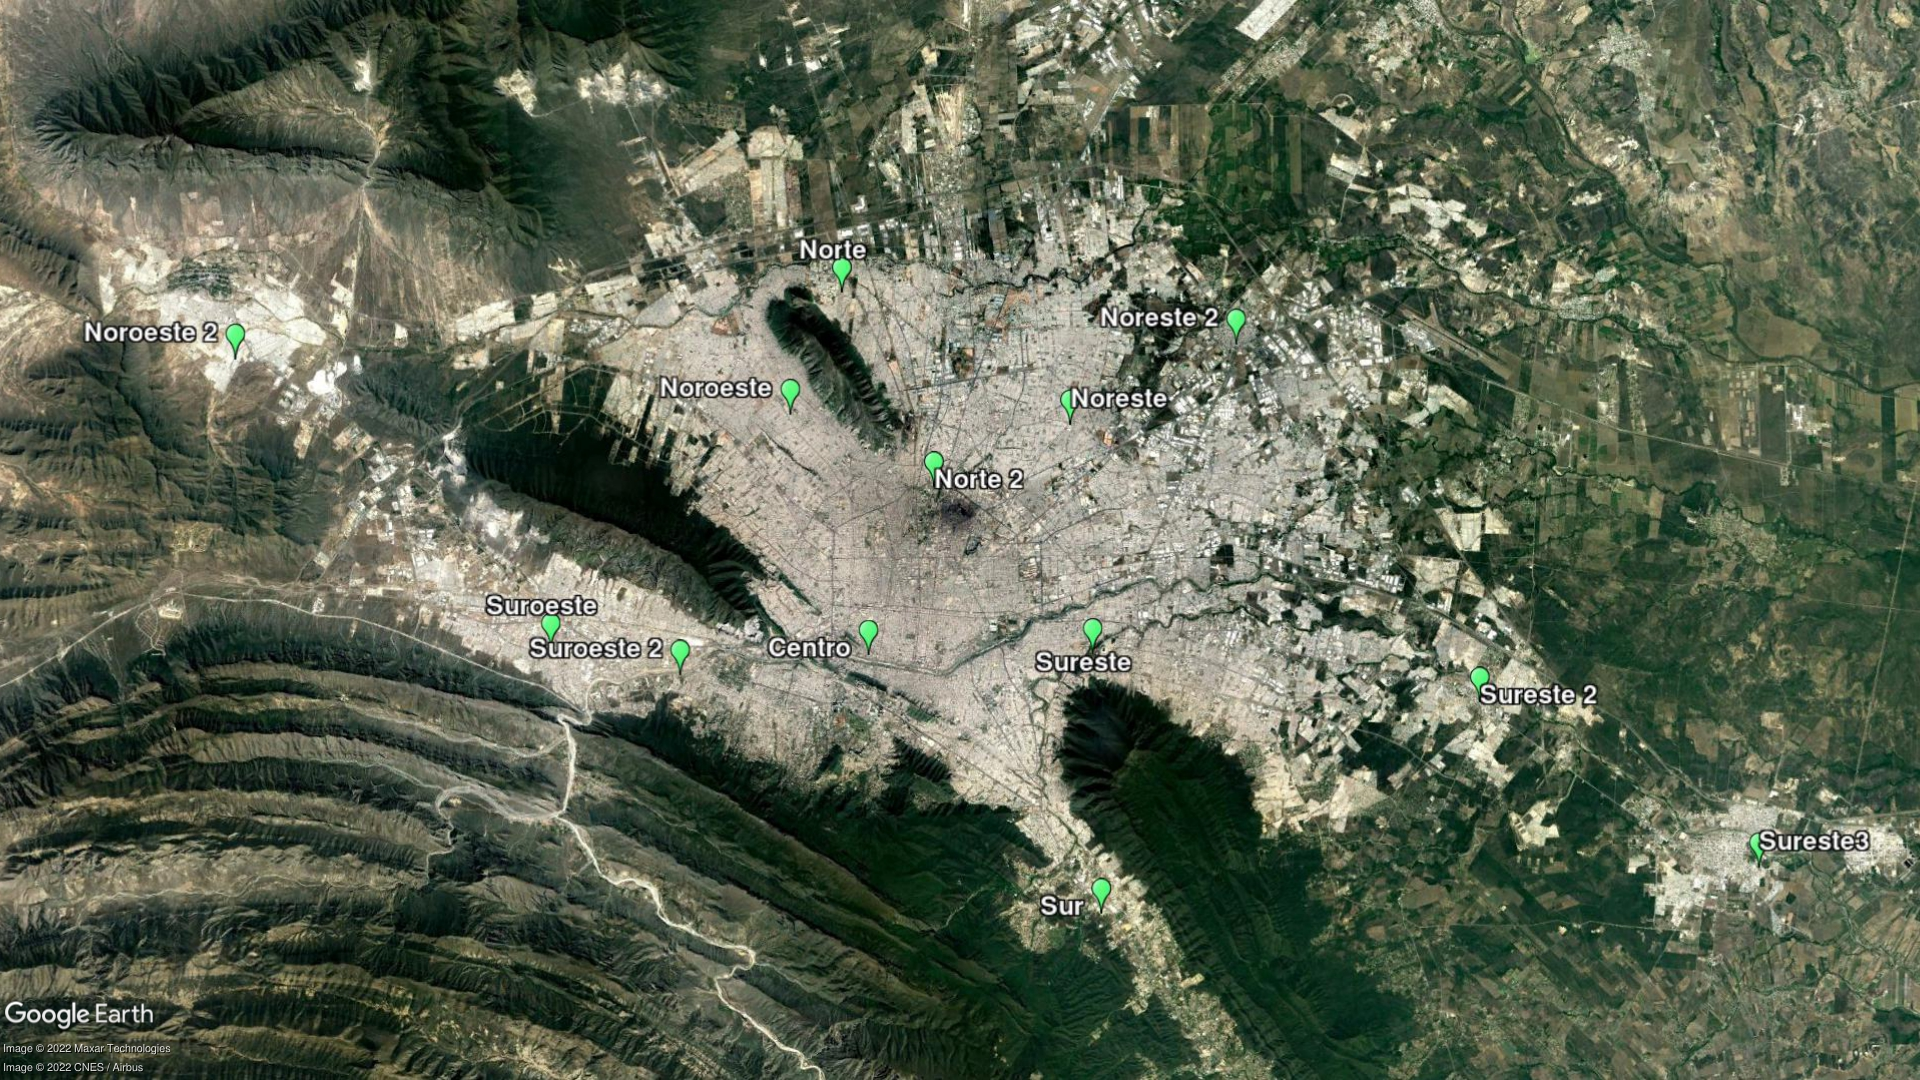
\includegraphics[width=14cm]{Graphics/map_nolabels.eps}
	\caption{Ubicación geográfica de las estaciones meteorológicas del SIMA en el AMM.}
	\label{fig:stations}
\end{figure}

En la tabla \ref{table:stations_information} se muestra la información geográfica de las estaciones meteorológicas del SIMA en el AMM.

\begin{table}[H]
	\footnotesize
	\centering
	\begin{tabular}{llcrrr} \hline
		\textbf{Ciudad}          & \textbf{Nombre} & \begin{tabular}{cc}														 \textbf{Elevación} \\\textbf{(m s. n. m.)}\end{tabular} & \textbf{Latitud (°N)} & \textbf{Longitud (°O)} \\ \hline
		Guadalupe                & Sureste         & 492                                                                                                                        & 25.6680               & -100.2490              \\
		Monterrey                & Centro          & 560                                                                                                                        & 25.6700               & -100.3380              \\
		Monterrey                & Noroeste        & 571                                                                                                                        & 25.7570               & -100.3660              \\
		San Nicolas de los Garza & Noreste         & 476                                                                                                                        & 25.7500               & -100.2550              \\
		Santa Catarina           & Suroeste        & 694                                                                                                                        & 25.6760               & -100.4640              \\
		Garcia                   & Noroeste2       & 716                                                                                                                        & 25.7830               & -100.5860              \\
		Escobedo                 & Norte           & 528                                                                                                                        & 25.8000               & -100.3440              \\
		Apodaca                  & Noreste2        & 432                                                                                                                        & 25.7770               & -100.1880              \\
		Juarez                   & Sureste2        & 387                                                                                                                        & 25.6460               & -100.0960              \\
		San Pedro Garza Garcia   & Suroeste2       & 636                                                                                                                        & 25.6650               & -100.4130              \\
		Cadereyta de Jimenez     & Sureste3        & 340                                                                                                                        & 25.5833               & -99.9872               \\
		Monterrey                & Sur             & 630                                                                                                                        & 25.5749               & -100.2489              \\
		San Nicolas de los Garza & Norte2          & 520                                                                                                                        & 25.7295               & -100.3099              \\ \hline
	\end{tabular}
	\caption{Información de la localización geográfica de las estaciones meteorológicas del SIMA en el AMM.}
	\label{table:stations_information}
\end{table}

Se conto con una base de datos que contiene mediciones de irradiancia solar por hora en las estaciones del SIMA en el periodo 1993-2021. Se realizo un conteo de los meses que cumplen las siguientes condiciones:

\begin{itemize}
	\item Un día valido es aquel que contiene al menos 10 mediciones en el periodo de las 8 a las 19 horas.
	\item Un mes valido es aquel que contiene al menos 21 días validos.
\end{itemize}

En la figura \ref{fig:distribution_data} se muestra la distribución de los meses validos en las estaciones del SIMA bajo las condiciones anteriores.

\begin{figure}[H]
	\centering
	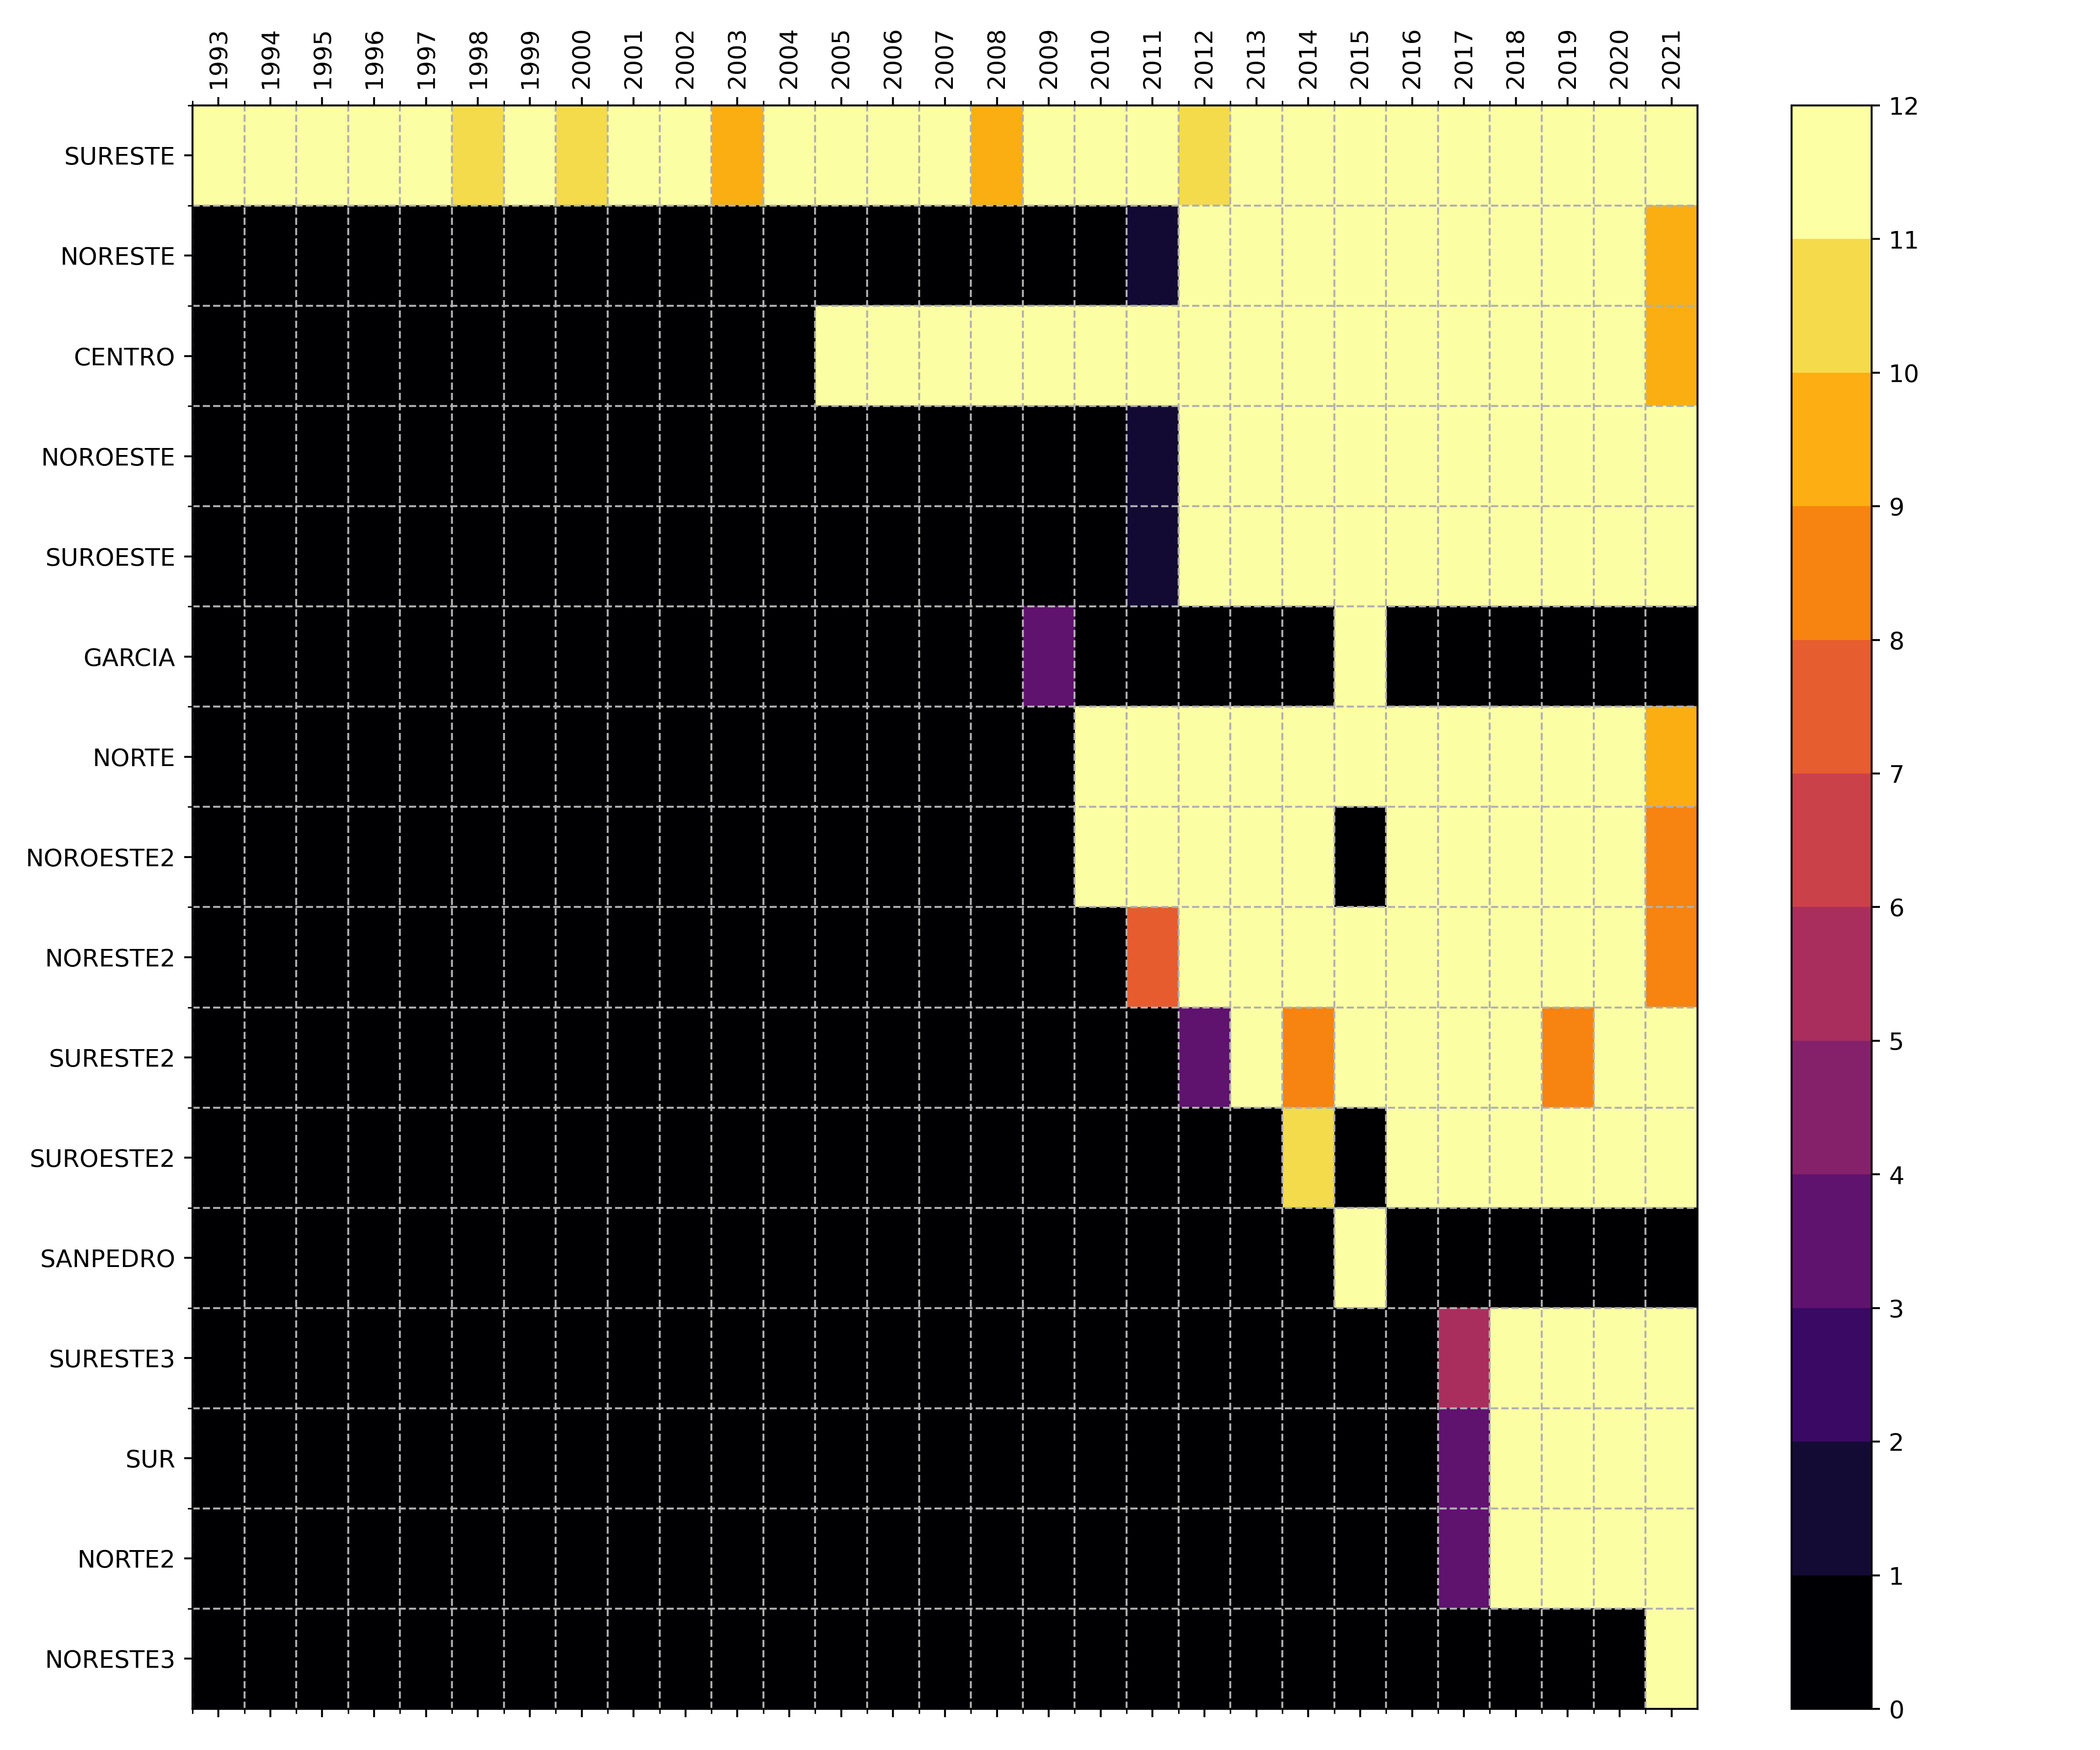
\includegraphics[width=11cm]{Graphics/Distribution_stations.png}
	\caption{Distribución de los meses validos para las estaciones meteorológicas del SIMA en el periodo 1993-2021.}
	\label{fig:distribution_data}
\end{figure}

\section{Creación de la base de datos}

Se seleccionaron las estaciones noroeste, noreste, sureste2 y suroeste en el periodo 2019-2021. Estas estaciones fueron elegidas debido a que la geografía alredeor es muy diferente y porque presentan un gran número de mediciones dentro del periodo seleccionado. En base a las mediciones diarias de cada estación se clasificó visualmente la condición de cielo para cada día. Las condiciones de cielo contempladas son despejado, parcialmente nublado y nublado.

\subsection{Criterios para las condiciones de cielo despejado}

Los criterios para la clasificación de cielo despjado de manera visual de las mediciones diarias son las siguientes:

\begin{itemize}
	\item Cielo despejado
		\begin{itemize}
			\item Un día de cielo despejado se caracteriza por tener un comportamiento gaussiano a lo largo del día, teniendo como máximo el mediodía solar. Para el AMM, el mediodía solar debe encontrarse alrededor de las 12:30-14:30 horas. Las mediciones deben registrar un valor diferente a cero entre las 6 a las 20 horas.
		\end{itemize}
	\item Cielo parcialmente nublado
		\begin{itemize}
			\item Un día de cielo parcialmente nublado se caracteriza por presentar el comportamiento de un día con cielo despejado pero en ciertos intervalos de tiempo. Esto puede ocurrir en solo una hora, o en varias. Si el día contiene entre uno y cinco mediciones que caracterizan a un día despejado, entonces el día será clasificado como parcialmente nublado.
		\end{itemize}
	\item Cielo nublado
		\begin{itemize}
			\item Un día nublado se caracteriza por presentar un comportamiento caótico o un comportamiento gaussiano pero con valores más bajos en comparación a un día de cielo despeajdo.
		\end{itemize}
\end{itemize}

En la figura \ref{fig:example_sky_conditions} se presentan diferentes mediciones para visualizar las diferentes clasificaciones de las condiciones de cielo.

\begin{figure}[H]
	\centering
	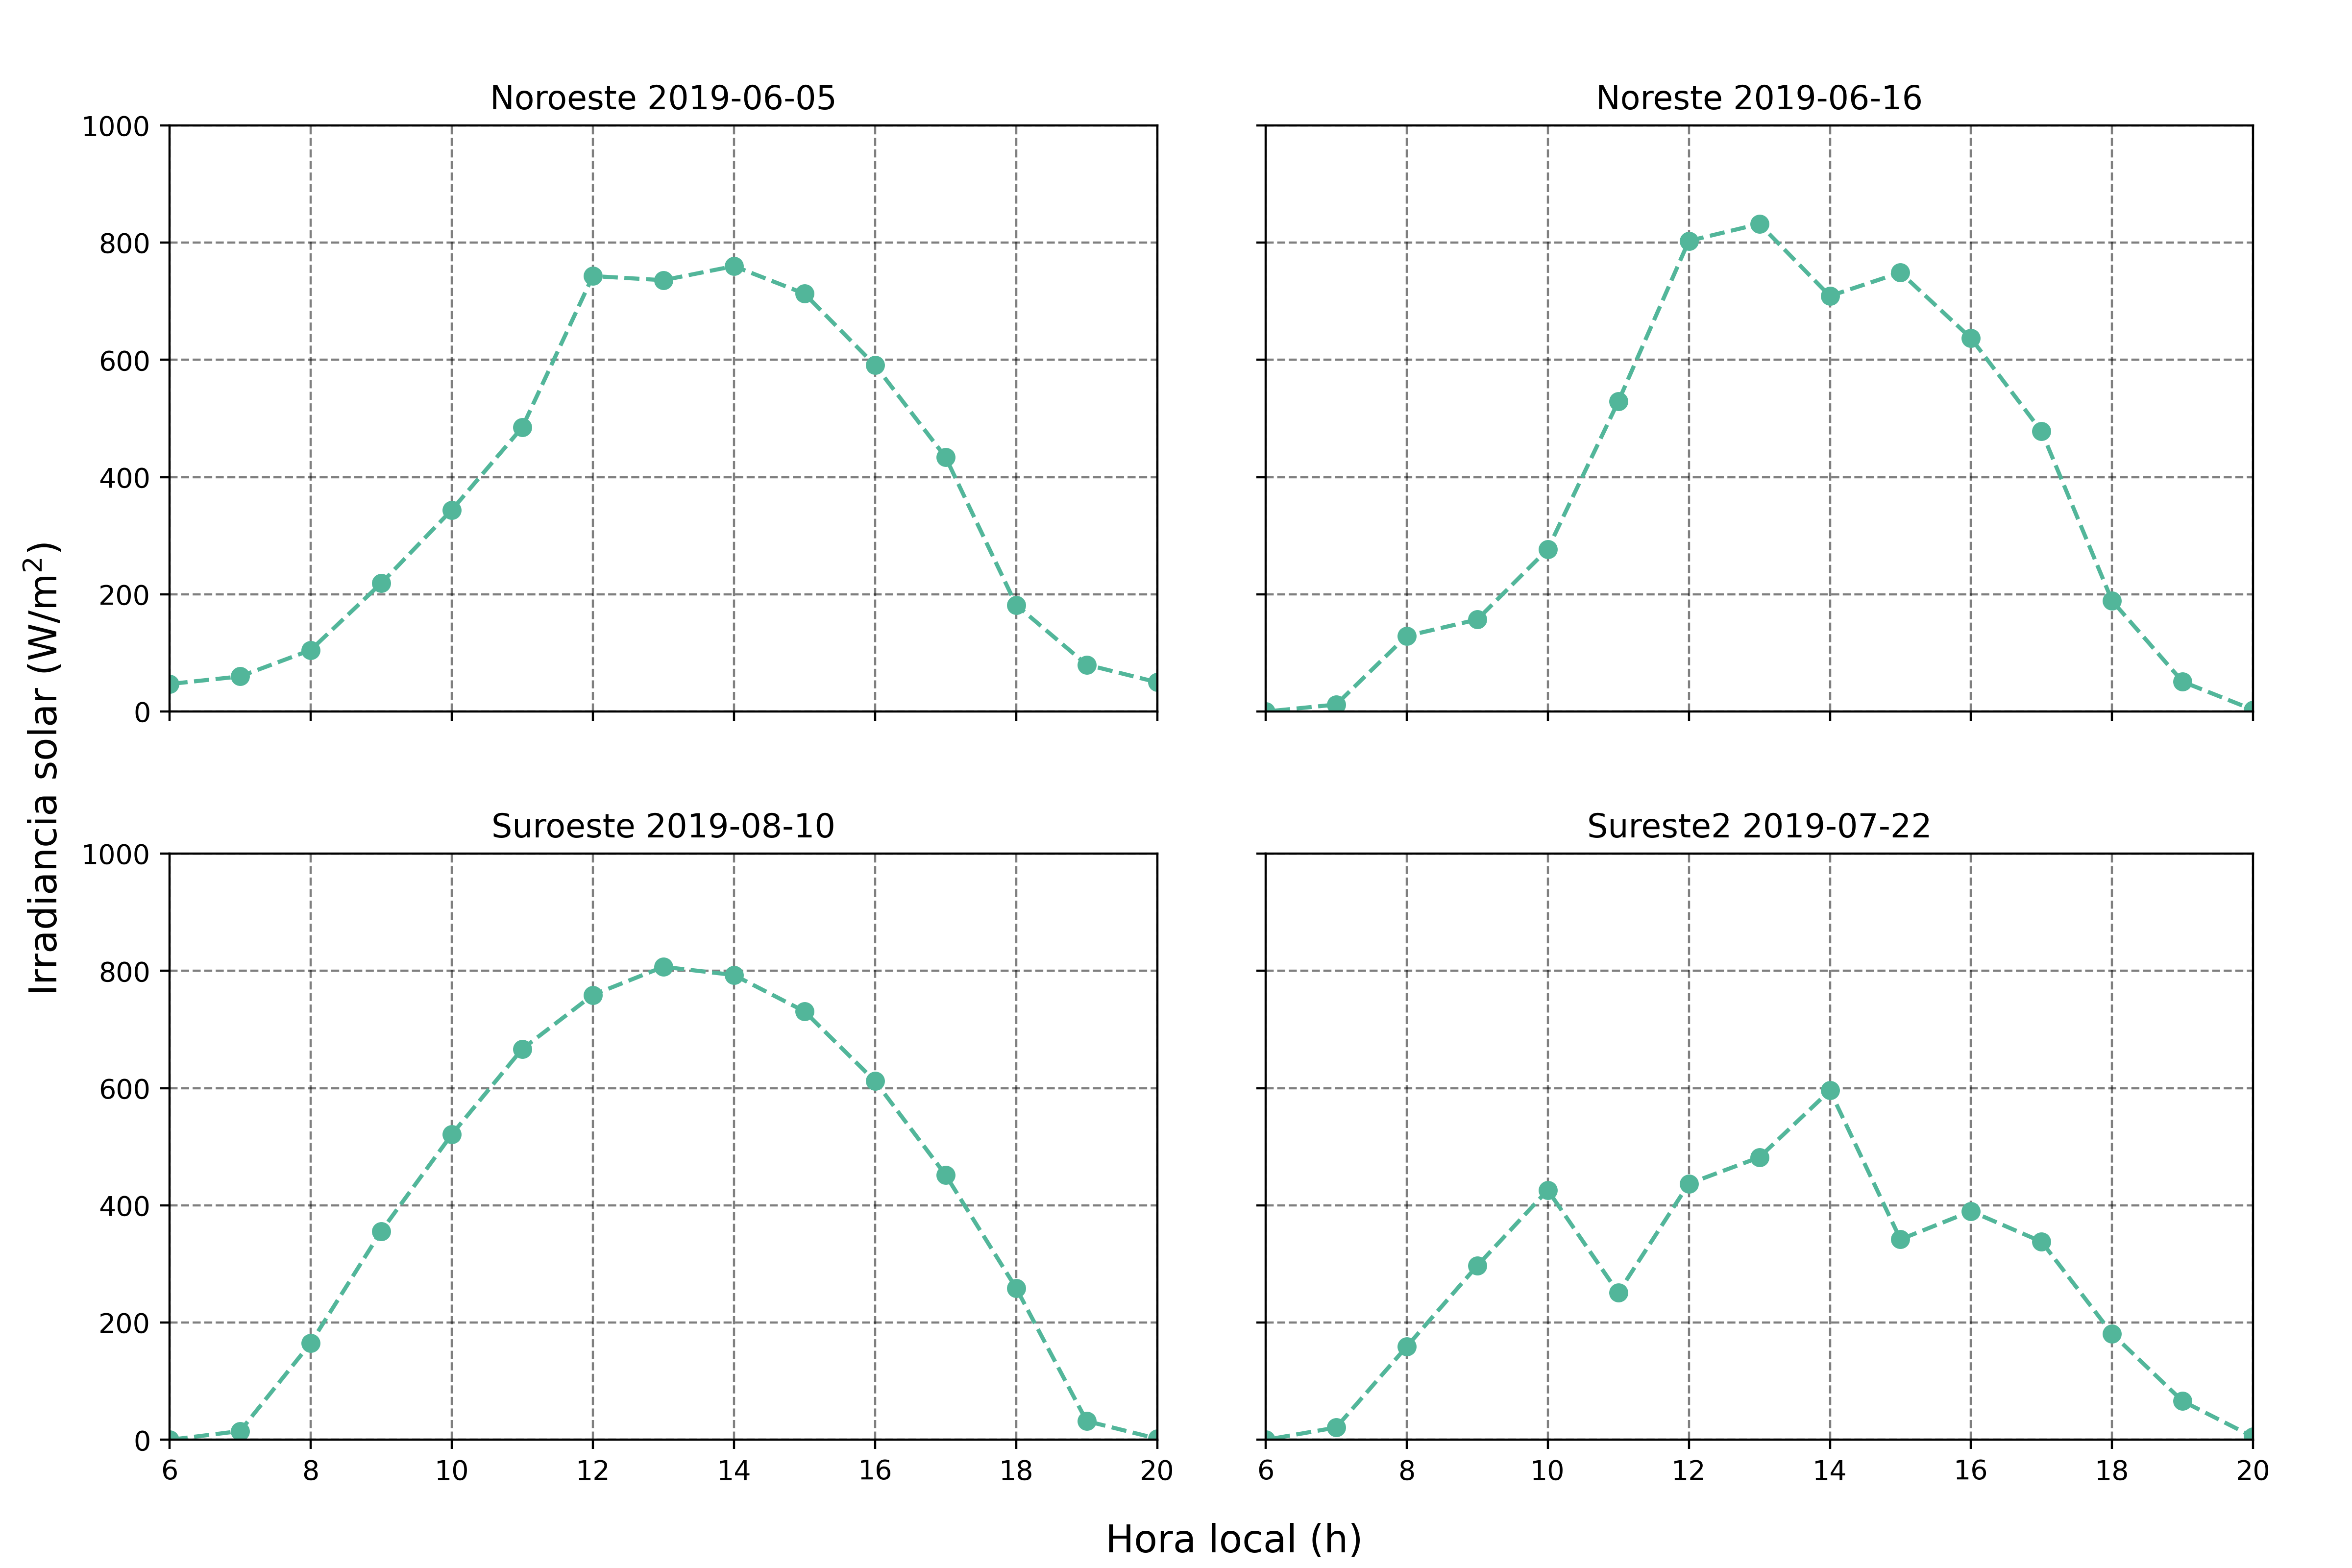
\includegraphics[width=15cm]{Graphics/example_sky_conditions.png}
	\caption{Ejemplos de las clasificaciones de las condiciones de cielo a partir de mediciones diarias de cada una de las estaciones del SIMA.}
	\label{fig:example_sky_conditions}
\end{figure}

\subsection{Datos atípicos}

Los datos de las estaciones del SIMA pueden contener ruido o mediciones que fisicamente no son posibles, a estos datos los denominamos como atípicos. Se implemento una limpieza de datos automática la cual consiste en realizar una operación de comparación para cada medición (ecuación \ref{eq:clean_comparison}) con respecto al modelo GHI, si esta operación para alguna hora es mayor a 0.9, entonces este valor corresponde a una medición atípco y se eliminará de la base de datos. Si el $k_t$ es igual a 0, entonces se sobreescribe la medición con el valor 0, esto con el propósito de eliminar el ruido que puede tener el radiometro de la estación analizada.

\begin{equation}
	k_t =\begin{cases}
		\frac{\text{Medición}}{\text{GHI}_0} & \text{si GHI}_0\neq 0 \\
		0                                    & \text{si GHI}_0 = 0
	\end{cases}
	\label{eq:clean_comparison}
\end{equation}

En la figura \ref{fig:example_clean_data} se visualiza en dos días diferentes el proceso de la limpieza de datos atípicos. Los valores atípicos ocurren con frecuencia al inicio o al final del día solar.

\begin{figure}[H]
	\centering
	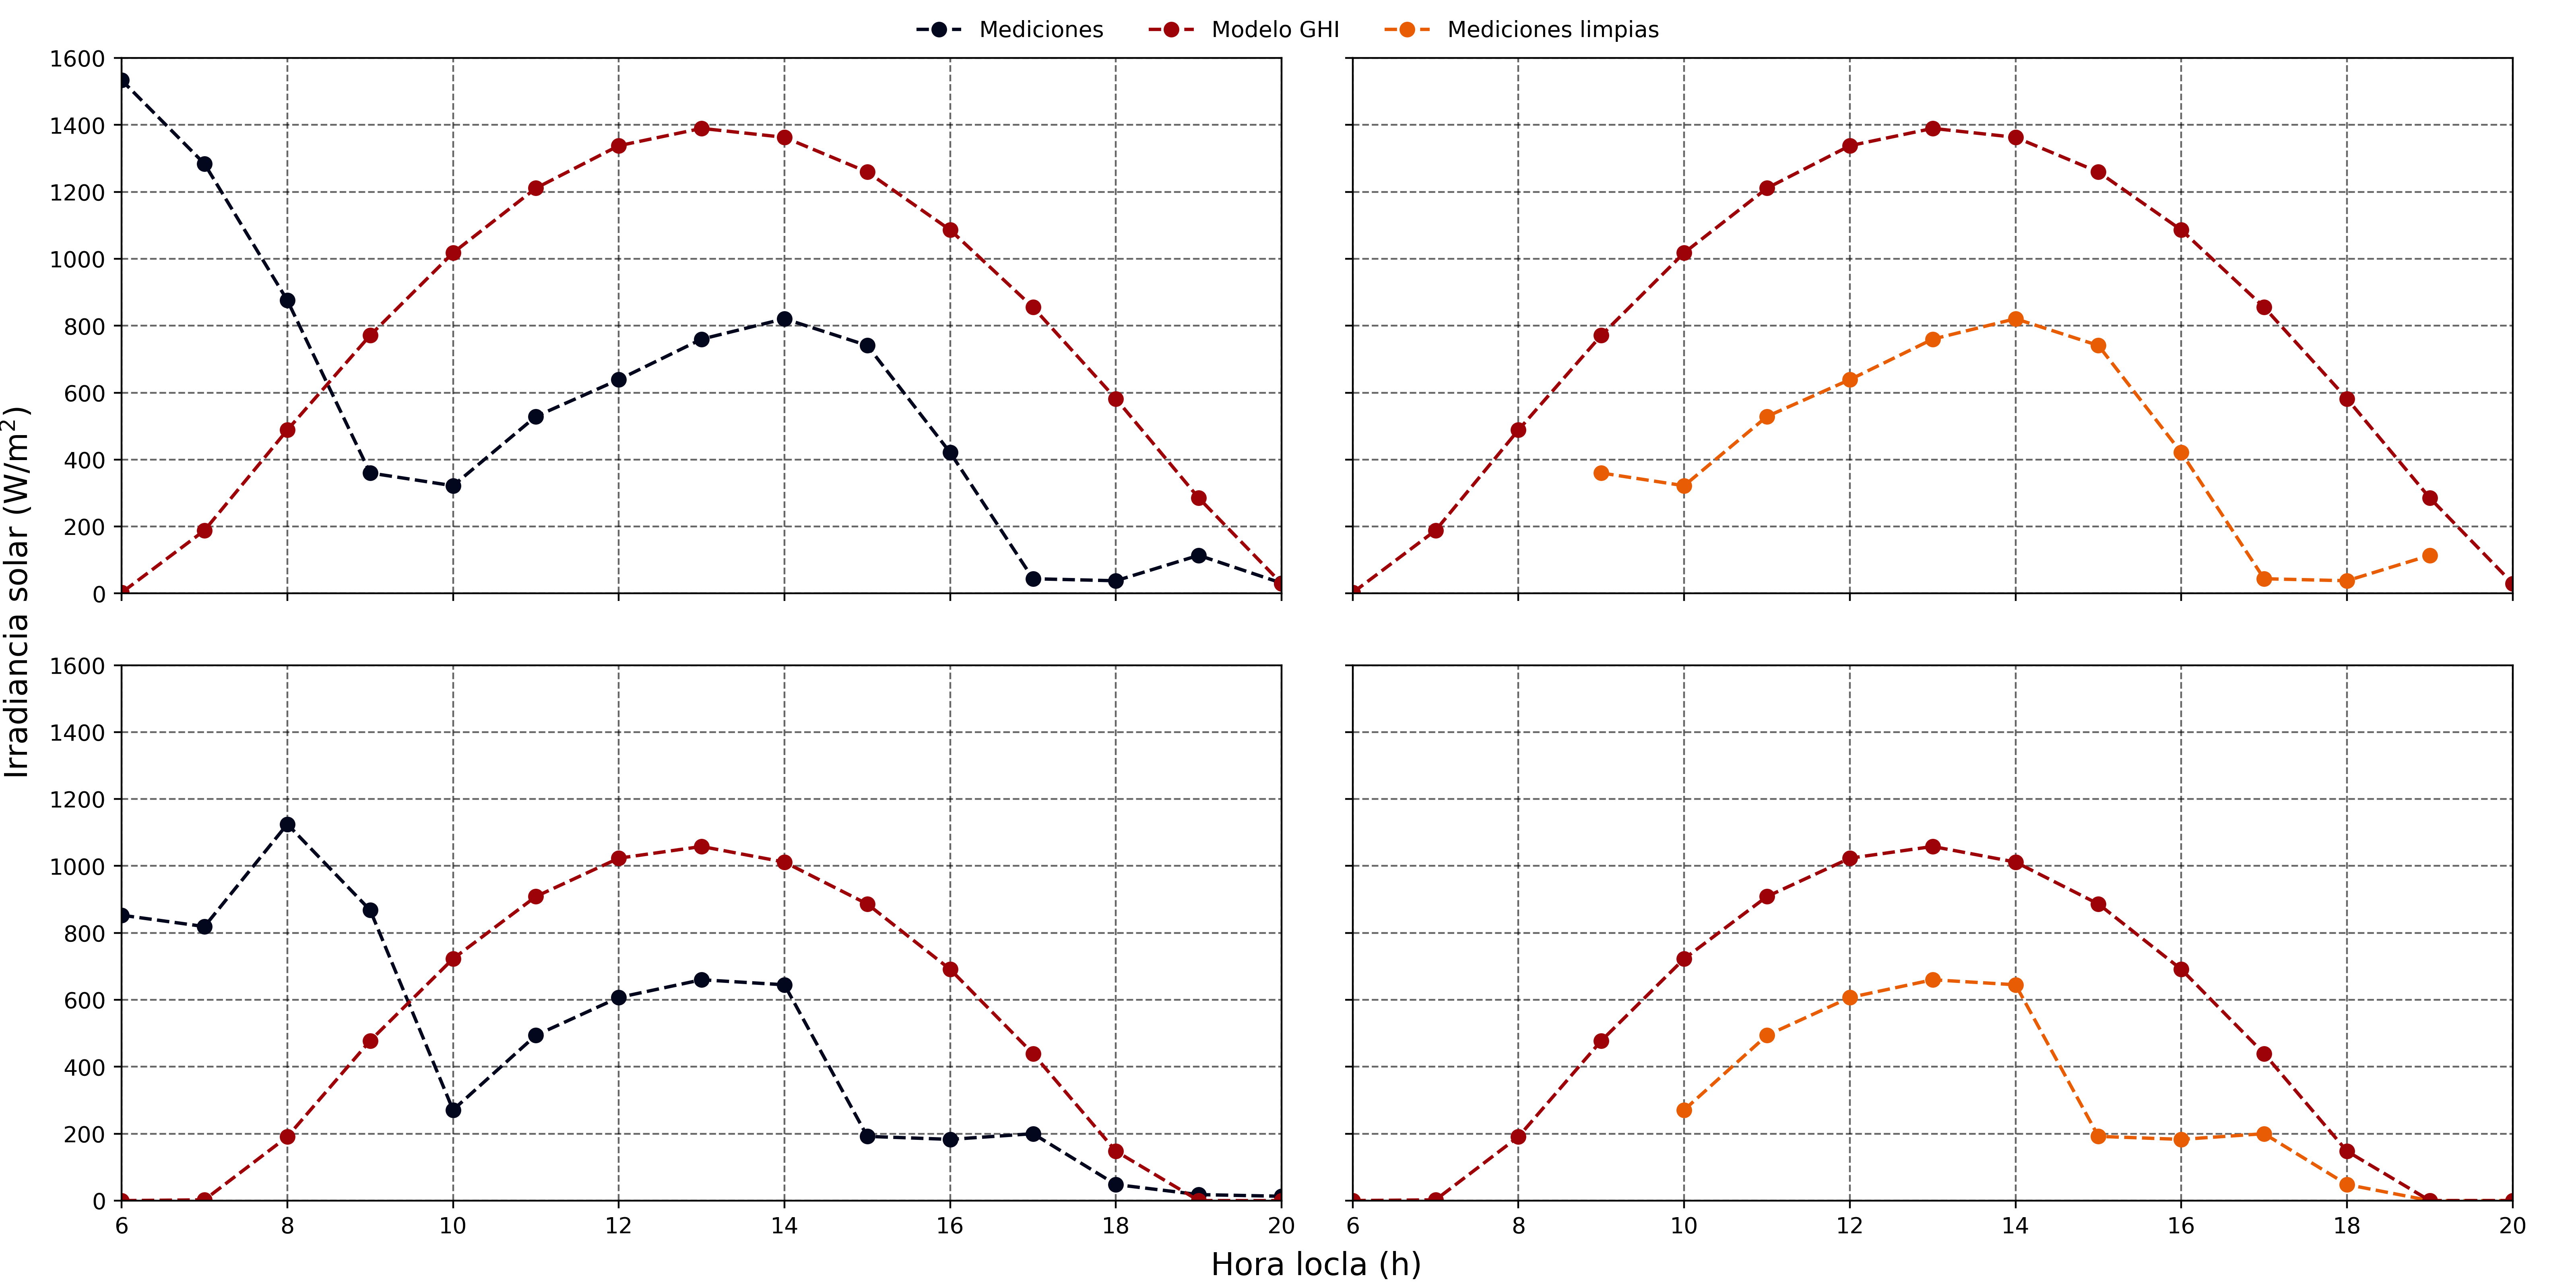
\includegraphics[width=15cm]{Graphics/example_clean_data.png}
	\caption{Mediciones de irradiancia solar de la estación noroeste originales (izquierda) y sin valores atípicos (derecha).}
	\label{fig:example_clean_data}
\end{figure}

\subsection{Reconstrucción}

A partir de los datos limpios, se aplico un proceso de reconstrucción. El proceso de reconstrucción consiste en asignar el valor del promedio horario de las 10 primeras mediciones que tengan más semejanza a la medición a reconstruir. Se toman unicamente las mediciones de la misma estación en una ventana de tres meses (un mes anterior, el mes actual y el siguiente). La semejanza se calcula en base a la similitud coseno (ecuación \ref{eq:cosine}).

\begin{equation}
	sim(m_i , m_j ) = \frac{m_i \cdot m_j}{||m_i|| ||m_j||}
	\label{eq:cosine}
\end{equation}

En la figura \ref{fig:restoration} se muestran los datos restaurados para los casos presentados en la figura \ref{fig:example_clean_data}.

\begin{figure}[H]
	\centering
	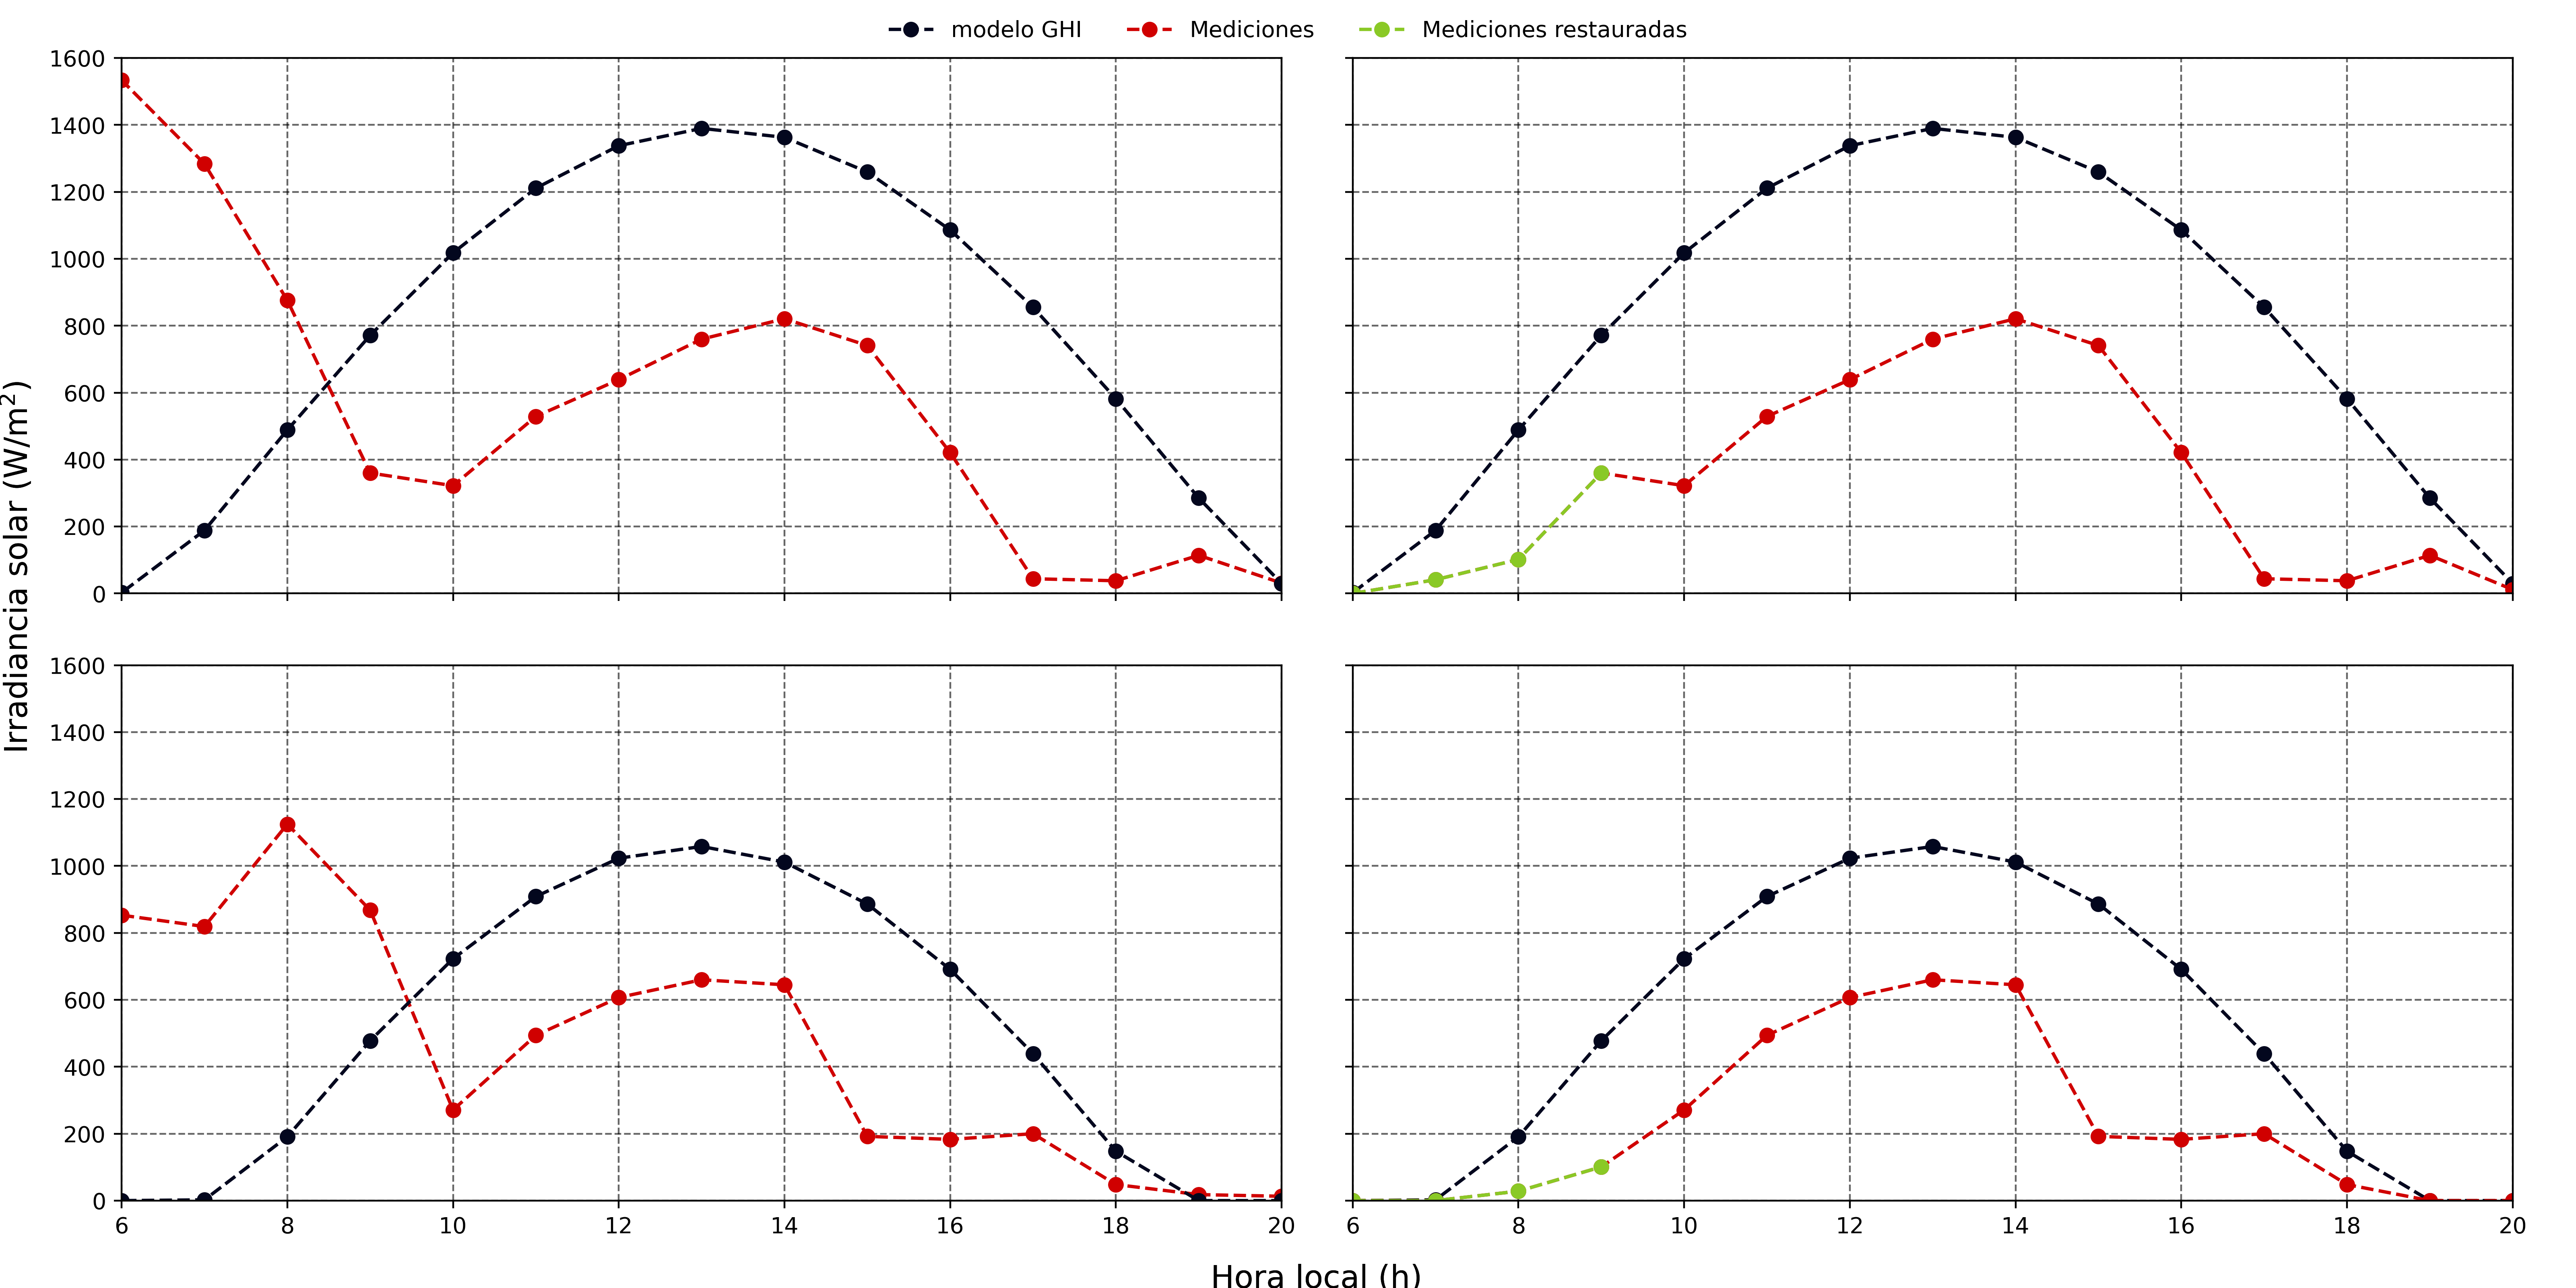
\includegraphics[width=15cm]{Graphics/example_restoration.png}
	\caption{Restauracion de mediciones por medio de promerios horarios de las 30 mediciones más semejantes al día seleccioando}
	\label{fig:restoration}
\end{figure}

Con las mediciones restauradas se realizaron las comparaciones (ecuación \ref{eq:diff} y ecuación \ref{eq:ratio}) con respecto a los modelos GHI$_0$ y RS.

\begin{equation}
	d_t = \begin{cases}
		\text{Modelo} - \text{Medición} & \text{si Modelo}\neq 0\\
		0 & \text{si Modelo} = 0
	\end{cases}
	\label{eq:diff}
\end{equation}

\begin{equation}
	k_t = \begin{cases}
		\frac{\text{Medición}}{\text{Modelo}} & \text{si Modelo}\neq 0\\
		0 & \text{si Modelo} = 0
	\end{cases}
	\label{eq:ratio}
\end{equation}
